\documentclass[tikz,border=6pt]{standalone}
\usepackage{amsmath,amssymb}
\usetikzlibrary{shapes.geometric,positioning,decorations.pathreplacing,calc}

\begin{document}
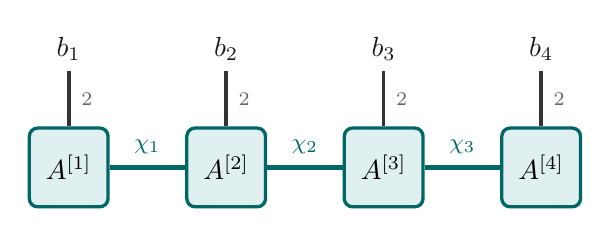
\begin{tikzpicture}[
    site/.style={draw=teal!80!black, fill=teal!12, rounded corners=3pt, line width=1.2pt, minimum size=1.0cm, align=center},
    leg/.style={line width=1.3pt, draw=black!80},
    bond/.style={line width=1.5pt, draw=teal!80!black},
    dimlabel/.style={font=\scriptsize\color{black!60}},
    indexlabel/.style={font=\normalsize\color{black!90}}
]

    % Sites
    \node[site] (A1) at (0, 0) {$A^{[1]}$};
    \node[site] (A2) at (2, 0) {$A^{[2]}$};
    \node[site] (A3) at (4, 0) {$A^{[3]}$};
    \node[site] (A4) at (6, 0) {$A^{[4]}$};

    % Virtual bonds
    \draw[bond] (A1.east) -- (A2.west) node[midway, above=1pt, font=\footnotesize\color{teal!80!black}] {$\chi_1$};
    \draw[bond] (A2.east) -- (A3.west) node[midway, above=1pt, font=\footnotesize\color{teal!80!black}] {$\chi_2$};
    \draw[bond] (A3.east) -- (A4.west) node[midway, above=1pt, font=\footnotesize\color{teal!80!black}] {$\chi_3$};

    % Physical legs
    \foreach \i/\nd in {1/A1, 2/A2, 3/A3, 4/A4} {
        \draw[leg] (\nd.north) -- ++(0, 0.7) node[above, indexlabel] {$b_\i$};
        \node[dimlabel, right=1pt] at ($(\nd.north) + (0, 0.35)$) {2};
    }

\end{tikzpicture}
\end{document}
